\section{Measurements of $\mathrm{V}_{cs}$ }

The CKM matrix originates from the Yukawa couplings in the SM Higgs sector. It represents the mixing between quarks' mass eigenstates and the flavor eigenstates. When physical quarks in their mass eigenstates participate in the weak interaction, they are projected to the flavor eigenstates by the corresponding element in the CKM matrix. More details about the CKM in the standard model are discussed in Section~\ref{sec:relatedWorks:qft:gws}. 

\begin{table}[ht]
    \centering
    \setlength{\tabcolsep}{1.5em}
    \renewcommand{\arraystretch}{1.5}
    \caption{The current experimental world average of the 9 elements in the CKM matrix in the PDG \cite{pdg2020}.  }
    \resizebox{\textwidth}{!}{
    \begin{tabular}{c|c|c }
        \hline
        $|V_{ud}|=0.97370 \pm 0.00014 $     & $|V_{us}|=0.2245 \pm 0.0008$      &  $|V_{ub}|=0.00382 \pm 0.00024$   \\ \hline
        $|V_{cd}|=0.221 \pm 0.004 $         & $|V_{cs}|=0.987 \pm 0.011$        &  $|V_{cb}|=0.0410 \pm 0.0014$     \\ \hline
        $|V_{td}|=0.0080 \pm 0.0003 $       & $|V_{ts}|=0.0388 \pm 0.0011$      &  $|V_{tb}|=1.013 \pm 0.030$       \\
        \hline
    \end{tabular}}
    \label{tab:relatedWorks:vcs:ckm}
\end{table}


The current experimental measurement of the 9 elements in the CKM matrix \cite{pdg2020} is shown in Table~\ref{tab:relatedWorks:vcs:ckm}. Among the 6 elements in the first two rows, \absVcs is measured with the least precision. The average of \absVcs measurements is shown in Figure~\ref{fig:relatedWorks:vcs:measurements}. Currently, there are two direct approaches to measure \absVcs, using the \PD meson decay in the charm factories and using the on-shell $W\to c s$  with jet tagging in the collider experiments.

The best direct determination of \absVcs is from the semileptonic decay of $D$ and the leptonic decay of \PDs produced in the charm factory. For the results from the leptonic decay of \PDs meson, the branching fraction of $\PDs^+ \to \mu^+ \nu$ and $\PDs^+ \to \tau^+ \nu$ are both measured in the Belle \cite{Zupanc:2013byn}, CLEO \cite{Alexander:2009ux,Onyisi:2009th,Naik:2009tk}, BaBar \cite{delAmoSanchez:2010jg} and BESIII \cite{Ablikim:2016duz, Ablikim:2018jun}. Using the experimental value of mass and lifetime of \PDs, as well as the lattice QCD calculation of the form factor $f_{\PDs}$, \absVcs can be determined from the \PDs leptonic decay and yields a world average of $\absVcs=0.992\pm 0.012$ \cite{Amhis:2019ckw}, where the dominating uncertainty is from the experimental error. For the results from the semileptonic decay of $D$ meson, the branching fraction of $D\to K l\nu$ is measured by CLEO-c \cite{Besson:2009uv}, Belle \cite{Widhalm:2006wz}, BaBar \cite{Aubert:2007wg} and BESIII \cite{Ablikim:2015ixa, Ablikim:2018evp}, which gives an average of \absVcs of $\absVcs=0.939\pm 0.038$ \cite{Amhis:2019ckw} in the \PD meson decay. The dominant uncertainty is form the theoretical calculations of the \PD meson form factor with latice QCD. Combining the result from the $D$ and \PDs decay, the charm factories measures $\absVcs=0.987\pm 0.011$ \cite{Amhis:2019ckw}.

The second direct measurement of \absVcs is from the on-shell $W\to c s$ decays in the collider experiments. This approach relies on jet tagging to identifies the jets originating from the c and s quarks, which is relatively difficult, especially in the hadron collider with a more complex hadron environment. Therefore, this approach is less explored compared with the $D/\PDs$ approach. So far, the only published result based on the $W\to c s$  approach is from the DELPHI in the LEP, which reports $\absVcs=0.94 ^{+0.32}_{-0.26}\pm 0.13$. \cite{Abreu:1998ap}

In Figure~\ref{fig:relatedWorks:vcs:measurements}, the indirect measurement of \absVcs is from the global fit by CKMFitter to all the measured CKM elements assuming the four SM parameters. In addition, LEP published another indirect result. LEP measures the $Br(W\to l \nu) = (10.83 \pm 0.07 \pm 0.07) \%$ \cite{Schael:2013ita}, based on which calculates the sum of all six CMK element in the first two rows as $\sum |V_{ij}|^2 = 2.002 \pm 0.027$. Since \absVcs is the least precisely measured element, LEP subtract other five elements from $|V_{ij}|^2 $ and produces an indirect measurement of $|V_{ij}|=0.969\pm 0.013$. This thesis measures the $Br(W\to l \nu) $ as well. Therefore, the same calculation as LEP can be done for our result to get \absVcs from $Br(W\to l \nu)$. The next part of this section covers about the steps of the such calculations.


 \begin{figure}
    \centering
%     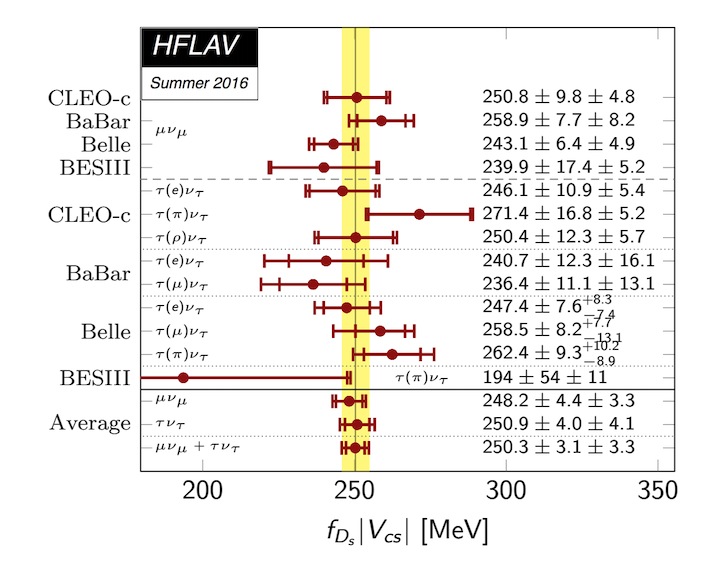
\includegraphics[width=0.45\textwidth]{vcs_meson_ds.png} \qquad
    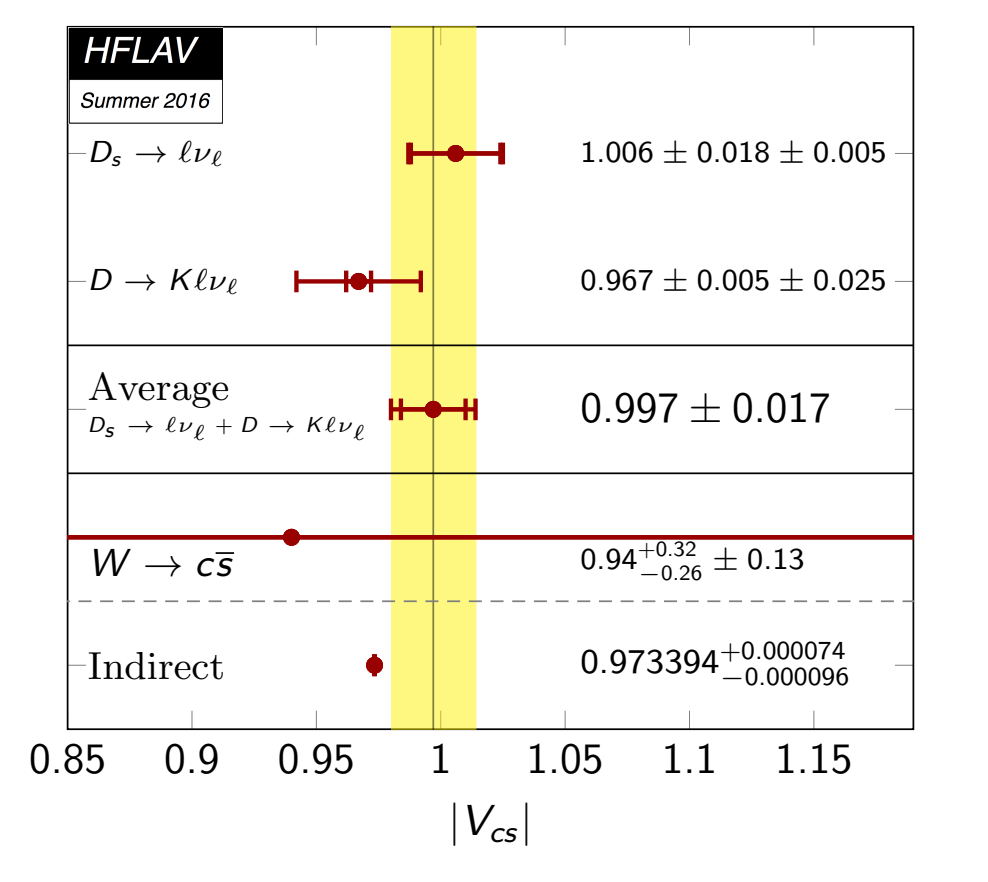
\includegraphics[width=0.6\textwidth]{chapters/RelatedWorks/sectionVcs/figures/vcs.png}
    \caption{The world average of \absVcs measurements. }
    \label{fig:relatedWorks:vcs:measurements}
\end{figure}
